\chapter{Results, Analysis and Discussion}\label{cha:Results Analysis and Discussion}
This chapter is a combined presentation of collected results, their analysis and a discussion. The first section is a presentation of the gathered results. 
The second section, divided into three subsections, introduces the evaluation of questions Q1, Q2 and Q3 respectively. The last section presents the 
conclusions of gathered data and performed analysis. 
\section{Results}
All results presented in this section are derived from two data sets. Each data set was collected separately. First data set is called variant 1 and the second is 
called variant 2. Both variants contain 2700 different maze problems, generated by Binary Tree, Aldous-Broder and Recursive-Backtracker
algorithms. \textcolor{red}{First variant is a data set of mazes with only one solution, variant 2 on the other hand contains mazes with more than one solution.} 
Each maze was a separate instance of a class Grid(), and the execution time of the solution was measured in the separated solver's method without the interference of
any additional process. For data collecting all visualisation features were disabled and all data were saved during each iteration to the .csv file.
\textcolor{red}{Variants produced  900 randomly applied sizes. However $27\%$ mazes} from variant 2 do not have a solution.To avoid a situation of a higher 
proportion of unsolvable mazes, there was applied a small, $3\%$, a ratio of directed cells, and a big, $50\%$ ratio of added connections between cells.
All data were collected on
MacBook Pro with an Apple M1 microchip, 8GB RAM and 11.6 macOS Big Sur operating system. All the figures used for analysis were made using the Python GUI application Orange v.3.33.
Each maze must fulfil the following presumptions:\\
$-$ two dimensional, minimum size 5$\times$5, maximum size 80$\times$80,\\
$-$ staring point coordinates [0,0], goal point [mazeSize.x - 1, mazeSize.y - 1],\\
$-$ weight of each edge equals 1.\\
\textbf{Variant 1 specific presumptions: }\\
$-$ perfect maze (Definition 20),\\
$-$ no directed edges,\\
$-$ each maze is solvable, there is a direct path from starting point to the goal point.\\
\textbf{Variant 2 specific presumptions: }\\
$-$ Unperfect maze (Definition 21),\\
$-$ $50\%$ of randomly added links to the randomly selected cells in a maze grid,\\
$-$ $3\%$ of south direction added to randomly selected cells in a maze grid,\\
$-$ mazes do not have to be solvable.\\
\subsection{Results}
\textcolor{red}{Majority of the presented results are characterized by high distribution skewness. For skewed distributions, the following values ​​are given in the tables:
average, SD, Median, Skewness, W (Shapiro-Wilk test result). For the presented scatter plots, different maze generators are distinguished by a different colour:
blue for the Aldous-Broder algorithm, red for the Recursive-Backtracker algorithm and green for the Binary Tree algorithm. The adopted confidence level is $\alpha = 0.05$ and 
the critical level of the test is $p<0.001$. A skewness lower than 1.5 is considered small. This indicates that the magnitude of the difference between the
sample distribution and the normal distribution is also small. A skewness higher than 1.5 is considered as medium or large, indicating a medium or large difference.}
%------------------------------------AVERAGE PATH LENGHT---------------------------------------------------------
\subsubsection{Paths Length}
Table 5.1 presents the results of the average and median of path length for generated mazes in variant 1.
According to Definition 8, paths in cyclic mazes may be infinite, therefore there is no data presented for variant 2. For Aldous-Broder and Binary Tree
generators, the average and SD may be considered as reliable measures due to the small skewness. However, for the Recursive-Backtracker the median is a more 
reliable measure due to the big skewness.
   
    \begin{table}[!ht]
        \centering
        \caption{Average and median of path length with a standard deviation of different maze generators.}
        \begin{tabular}{c c c c c c}
        \hline
            Maze Generator & Average & SD & Median & Skewness & W\\ \hline
            Aldous-Broder & 103 & 52 & 99 & 0.0775 & 0.960\\ 
            Binary Tre & 59 & 25 & 57 & 0.329 & 0.982\\ 
            Recursive-Backtracker & 311 & 227 & 263 & 1.469 & 0.880\\ \hline
        \end{tabular}
    \end{table}
%------------------------------------STEPS TO SOLVE---------------------------------------------------------
\subsubsection{Steps to solve}
Tables 5.2 and 5.3 present descriptive statistics of steps needed to solve a maze. Data is split by the maze generators and maze solvers. 
\begin{table}[!ht]
    \centering
    \caption{Variant 1: average and median of a number of steps needed to solve different maze generators by different maze solvers.} 
    \begin{tabular}{c c c c c c c}
    \hline
        Maze Solver & Maze Generator & Average & SD & Median & Skewness & W\\ \hline
        ~ & Aldous-Broder & 592 & 557 & 434.5 & 2.155 & 0.776\\ 
        Astar & Binary Tre & 77 & 30 & 80 & 0.066 & 0.989 \\ 
        ~ & Recursive-Backtracker & 972 & 893 & 711 & 1.670 & 0.832\\ \hline
        ~ & Aldous-Broder & 1170 & 949 & 956 & 1.261 & 0.890\\ 
        BFS & Binary Tre & 807 & 753 & 574 & 1.131 & 0.864\\ 
        ~ & Recursive-Backtracker & 1227 & 1037 & 958 & 1.264 & 0.874\\ \hline
        ~ & Aldous-Broder & 1773 & 1366 & 1361 & 0.862 & 0.916\\ 
        Dijkstra & Binary Tre & 1546 & 1254 & 1181 & 1.144 & 0.894\\ 
        ~ & Recursive-Backtracker & 1802 & 1343 & 1455 & 0.811 & 0.920\\ \hline
    \end{tabular}
\end{table}

\begin{table}[!ht]
    \centering
    \caption{\textcolor{red}{Variant 2: average and a median number of steps needed to solve different maze generators by different maze solvers.}}
    \begin{tabular}{c c c c c c c}
    \hline
        Maze Solver & Maze Generator & Average & SD & Median & Skewness & W\\ \hline
        ~ & Aldous-Broder & 155 & 67 & 153 & 0.359 & 0.989\\ 
        Astar & Binary Tre & 94 & 43 & 91 & 0.666 & 0.973 \\ 
        ~ & Recursive-Backtracker & 163 & 74 & 156 & 0.540 & 0.982\\ \hline
        ~ & Aldous-Broder & 973 & 875 & 689 & 1.500 & 0.848 \\ 
        BFS & Binary Tre & 709 & 810 & 428 & 2.366 & 0.717 \\ 
        ~ & Recursive-Backtracker & 979 & 890 & 715 & 1.647 & 0.840 \\ \hline
        ~ & Aldous-Broder & 1242 & 1118 & 800 & 1.268 & 0.865\\ 
        Dijkstra & Binary Tre & 1183 & 1066 & 840 & 1.418 & 0.852\\ 
        ~ & Recursive-Backtracker & 1148 & 1065 & 826 & 1.713 & 0.832\\ \hline
    \end{tabular}
\end{table}    
    %------------------------------------SOLUTION TIME---------------------------------------------------------
\subsubsection{Solution Time}
Figure 5.1, Table 5.4 and Table 5.5 presents an overview of the descriptive statistics of measured solution time.\\
\begin{figure}[!h]
    \centering
    \begin{subfigure}[b]{0.7\textwidth}
        \centering
        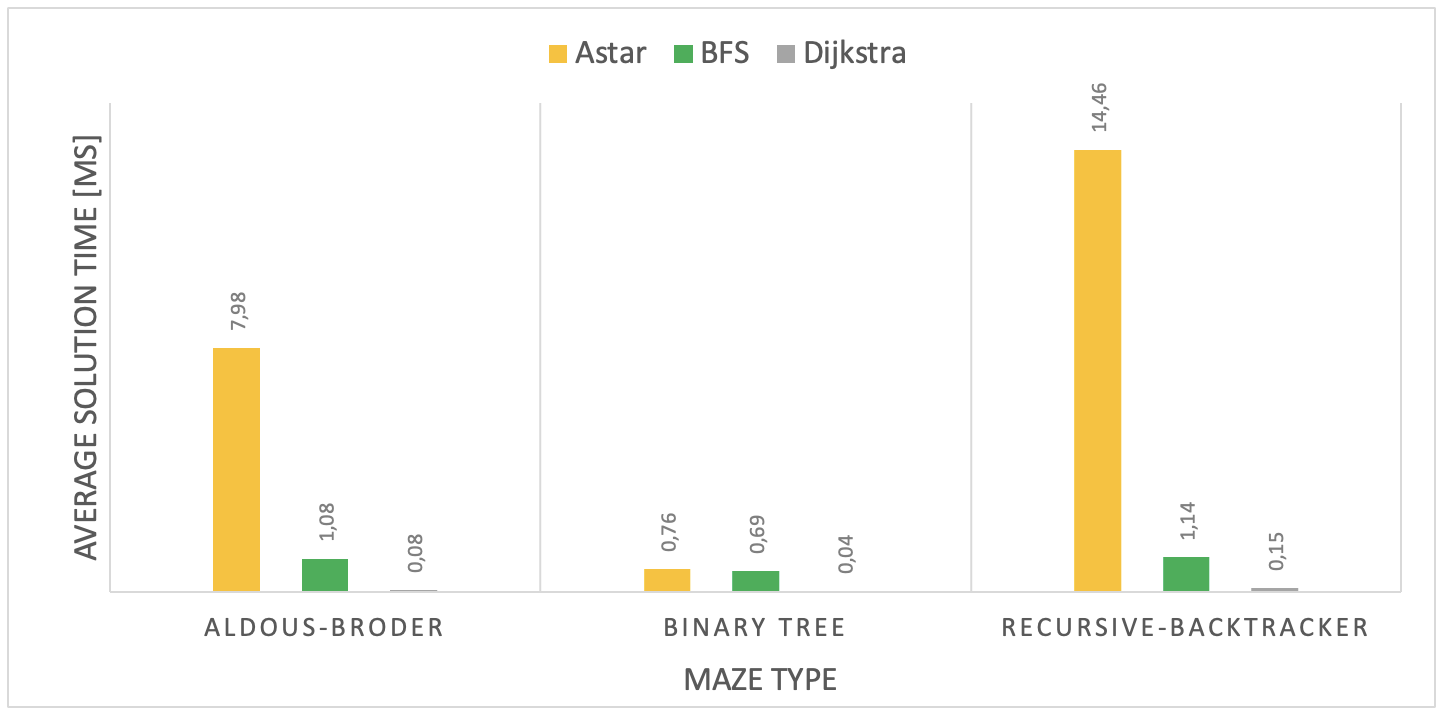
\includegraphics[width=\textwidth]{averagetime_variant1.png}
        \caption{}
    \end{subfigure}
    \begin{subfigure}[b]{0.7\textwidth}  
        \centering 
        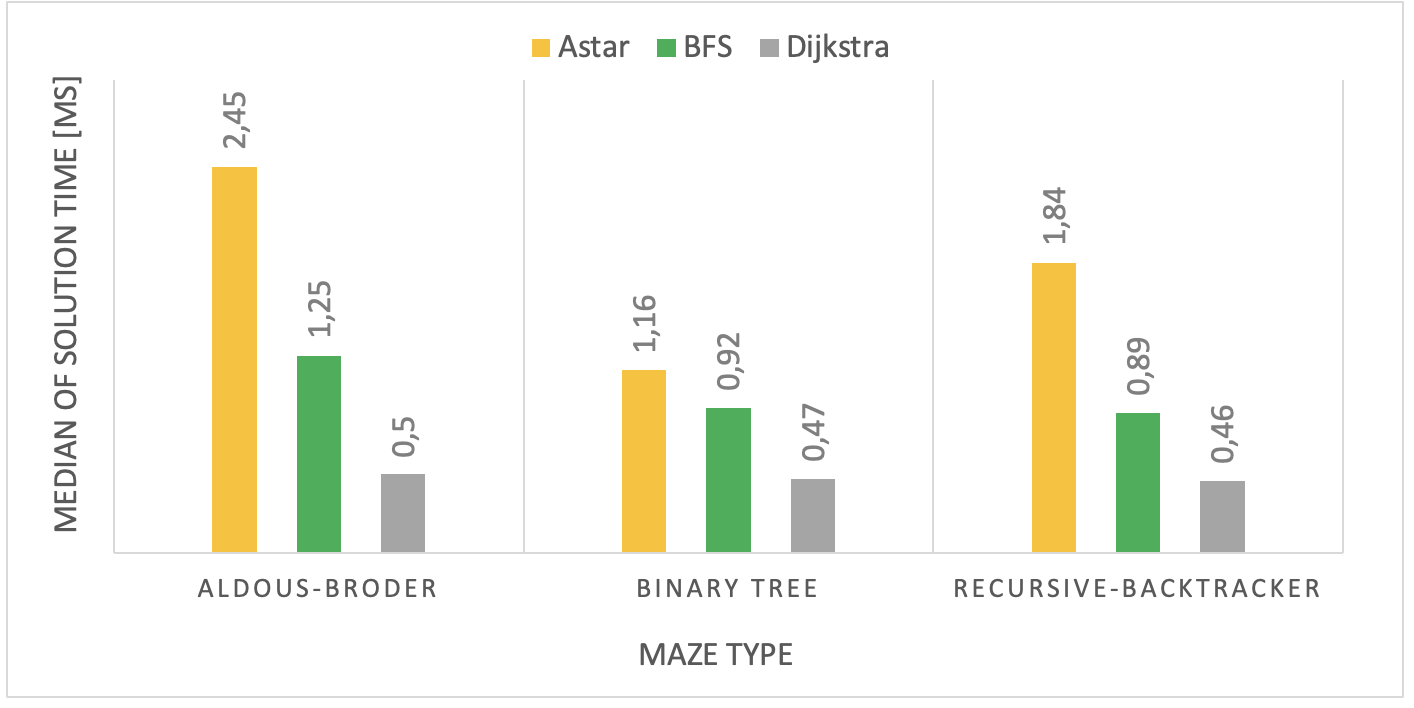
\includegraphics[width=\textwidth]{averagetime_variant2.png}
        \caption{}
    \end{subfigure}
    \caption[]{(a) presents Variant 1 and (b) presents Variant 2: mean solution time for different maze generators solved by different maze solvers.}
\end{figure}
%-----------------SOLUTION TIME VARIANT 1 TABLE-----------------------------------------------
\begin{table}[!ht]
    \centering
    \caption{Variant 1: Descriptive statistics of solution time for different maze solvers of different maze generators.} 
    \begin{tabular}{c c c c c c c}
    \hline
        Maze Solver & Maze Generator & Average & SD & Median & Skewness & W \\ \hline
        ~ & Aldous-Broder  & 20.74 & 40.08 & 7.98 & 3.96 & 0.493\\ 
        Astar & Binary Tree & 1.33 & 1.24 & 0.76 & 1.57 & 0.817\\ 
        ~ & Recursive-Backtracker & 47.10 & 83.67 & 14.46 & 3.40 & 0.575\\ \hline
        ~ & Aldous-Broder  & 1.29 & 1.05 & 1.08 & 1.57 & 0.886\\ 
        BFS & Binary Tree & 0.92 & 1.13 & 0.69 & 7.07 & 0.578\\ 
        ~ & Recursive-Backtracker & 1.38 & 1.18 & 1.14 & 2.03 & 0.853\\ \hline
        ~ & Aldous-Broder  & 0.11 & 0.10 & 0.08 & 1.99 & 0.743\\ 
        Dijkstra & Binary Tree & 0.08 & 0.09 & 0.04 & 1.80 & 0.663\\ 
        ~ & Recursive-Backtracker & 0.20 & 0.24 & 0.15 & 6.70 & 0.533 \\ \hline
    \end{tabular}
\end{table}

%-----------------SOLUTION TIME VARIANT 2 TABLE-----------------------------------------------
         \begin{table}[!ht]
            \centering
            \caption{Variant 2: Descriptive statistics of solution time for different maze solvers of different maze generators.} 
            \begin{tabular}{c c c c c c c}
            \hline
                Maze Solver & Maze Generator & Average & SD & Median & Skewness & W\\ \hline
                ~ & Aldous-Broder  & 2.52 & 1.68 & 2.45 & 0.73 & 0.955\\ 
                Astar & Binary Tree & 1.41 & 1.08 & 1.16 & 0.79 & 0.917\\ 
                ~ & Recursive-Backtracker & 2.20 & 1.67 & 1.84 & 1.25 & 0.908\\ \hline
                ~ & Aldous-Broder  & 1.35 & 1.07 & 1.25 & 0.87 & 0.923\\ 
                BFS & Binary Tree & 1.07 & 0.99 & 0.92 & 1.87 & 0.845 \\ 
                ~ & Recursive-Backtracker & 1.19 & 1.06 & 0.89 & 1.29 & 0.876\\ \hline
                ~ & Aldous-Broder & 0.72 & 0.64 & 0.50 & 1.53 & 0.846 \\ 
                Dijkstra & Binary Tree & 0.71 & 0.71 & 0.47 & 2.77 & 0.759\\ 
                ~ & Recursive-Backtracker & 0.64 & 0.58 & 0.46 & 1.91 & 0.815 \\ \hline
            \end{tabular}
        \end{table}
      %------------------------------------MCCLENDON'S--------------------------------------------------------
\newpage
      \subsubsection{McClendon's complexity}
Tables 5.6 and 5.7 present the average and median of the complexity measure for different maze generators. Modulo of skewness is lower than 1.5 which states the set
distribution is very close to the normal distribution, therefore, the average and SD may be considered the reliable measure. Figures 5.2a and 5.3a present scatter
plots of maze size versus McClendon's complexity. In Figures, 5.2a and 5.2b, a box plot of McClendon's complexity distributions are showing
mean complexity with standard deviation and maximal and minimal values.\\
\begin{table}[!ht]
    \centering
    \caption{Variant 1: Descriptive statistics of McClendon's complexity for different maze generators.} 
    \begin{tabular}{c c c c c c}
    \hline
        Maze Generator & Average & SD & Median & Skewness & W  \\ \hline
        Aldous-Broder & 13.83 & 2.12 & 14.13 & -0.67 & 0.965  \\ 
        Binary Tree  & 11.36 & 1.98 & 11.49 & -0.51 & 0.972 \\ 
        Recursive-Backtracker  & 14.94 & 2.48 & 15.39 & -0.58 & 0.971 \\ \hline
    \end{tabular}
\end{table}  

\begin{table}[!ht]
    \centering
    \caption{Variant 2: Descriptive statistics of McClendon's complexity for different maze generators.} 
    \begin{tabular}{c c c c c c}
    \hline
        Maze Generator & Average & SD & Median & Skewness & W  \\ \hline
        Aldous-Broder & 11.61 & 1.78 & 11.92 & -0.96 & 0.944  \\ 
        Binary Tree & 10.72 & 1.91 & 11.00 & -0.55 & 0.964  \\ 
        Recursive-Backtracker & 10.78 & 1.77 & 11.05 & -0.82 & 0.956  \\ \hline
    \end{tabular}
\end{table}

        \begin{figure}[!h]
            \centering
            \begin{subfigure}[!h]{0.7\textwidth}
               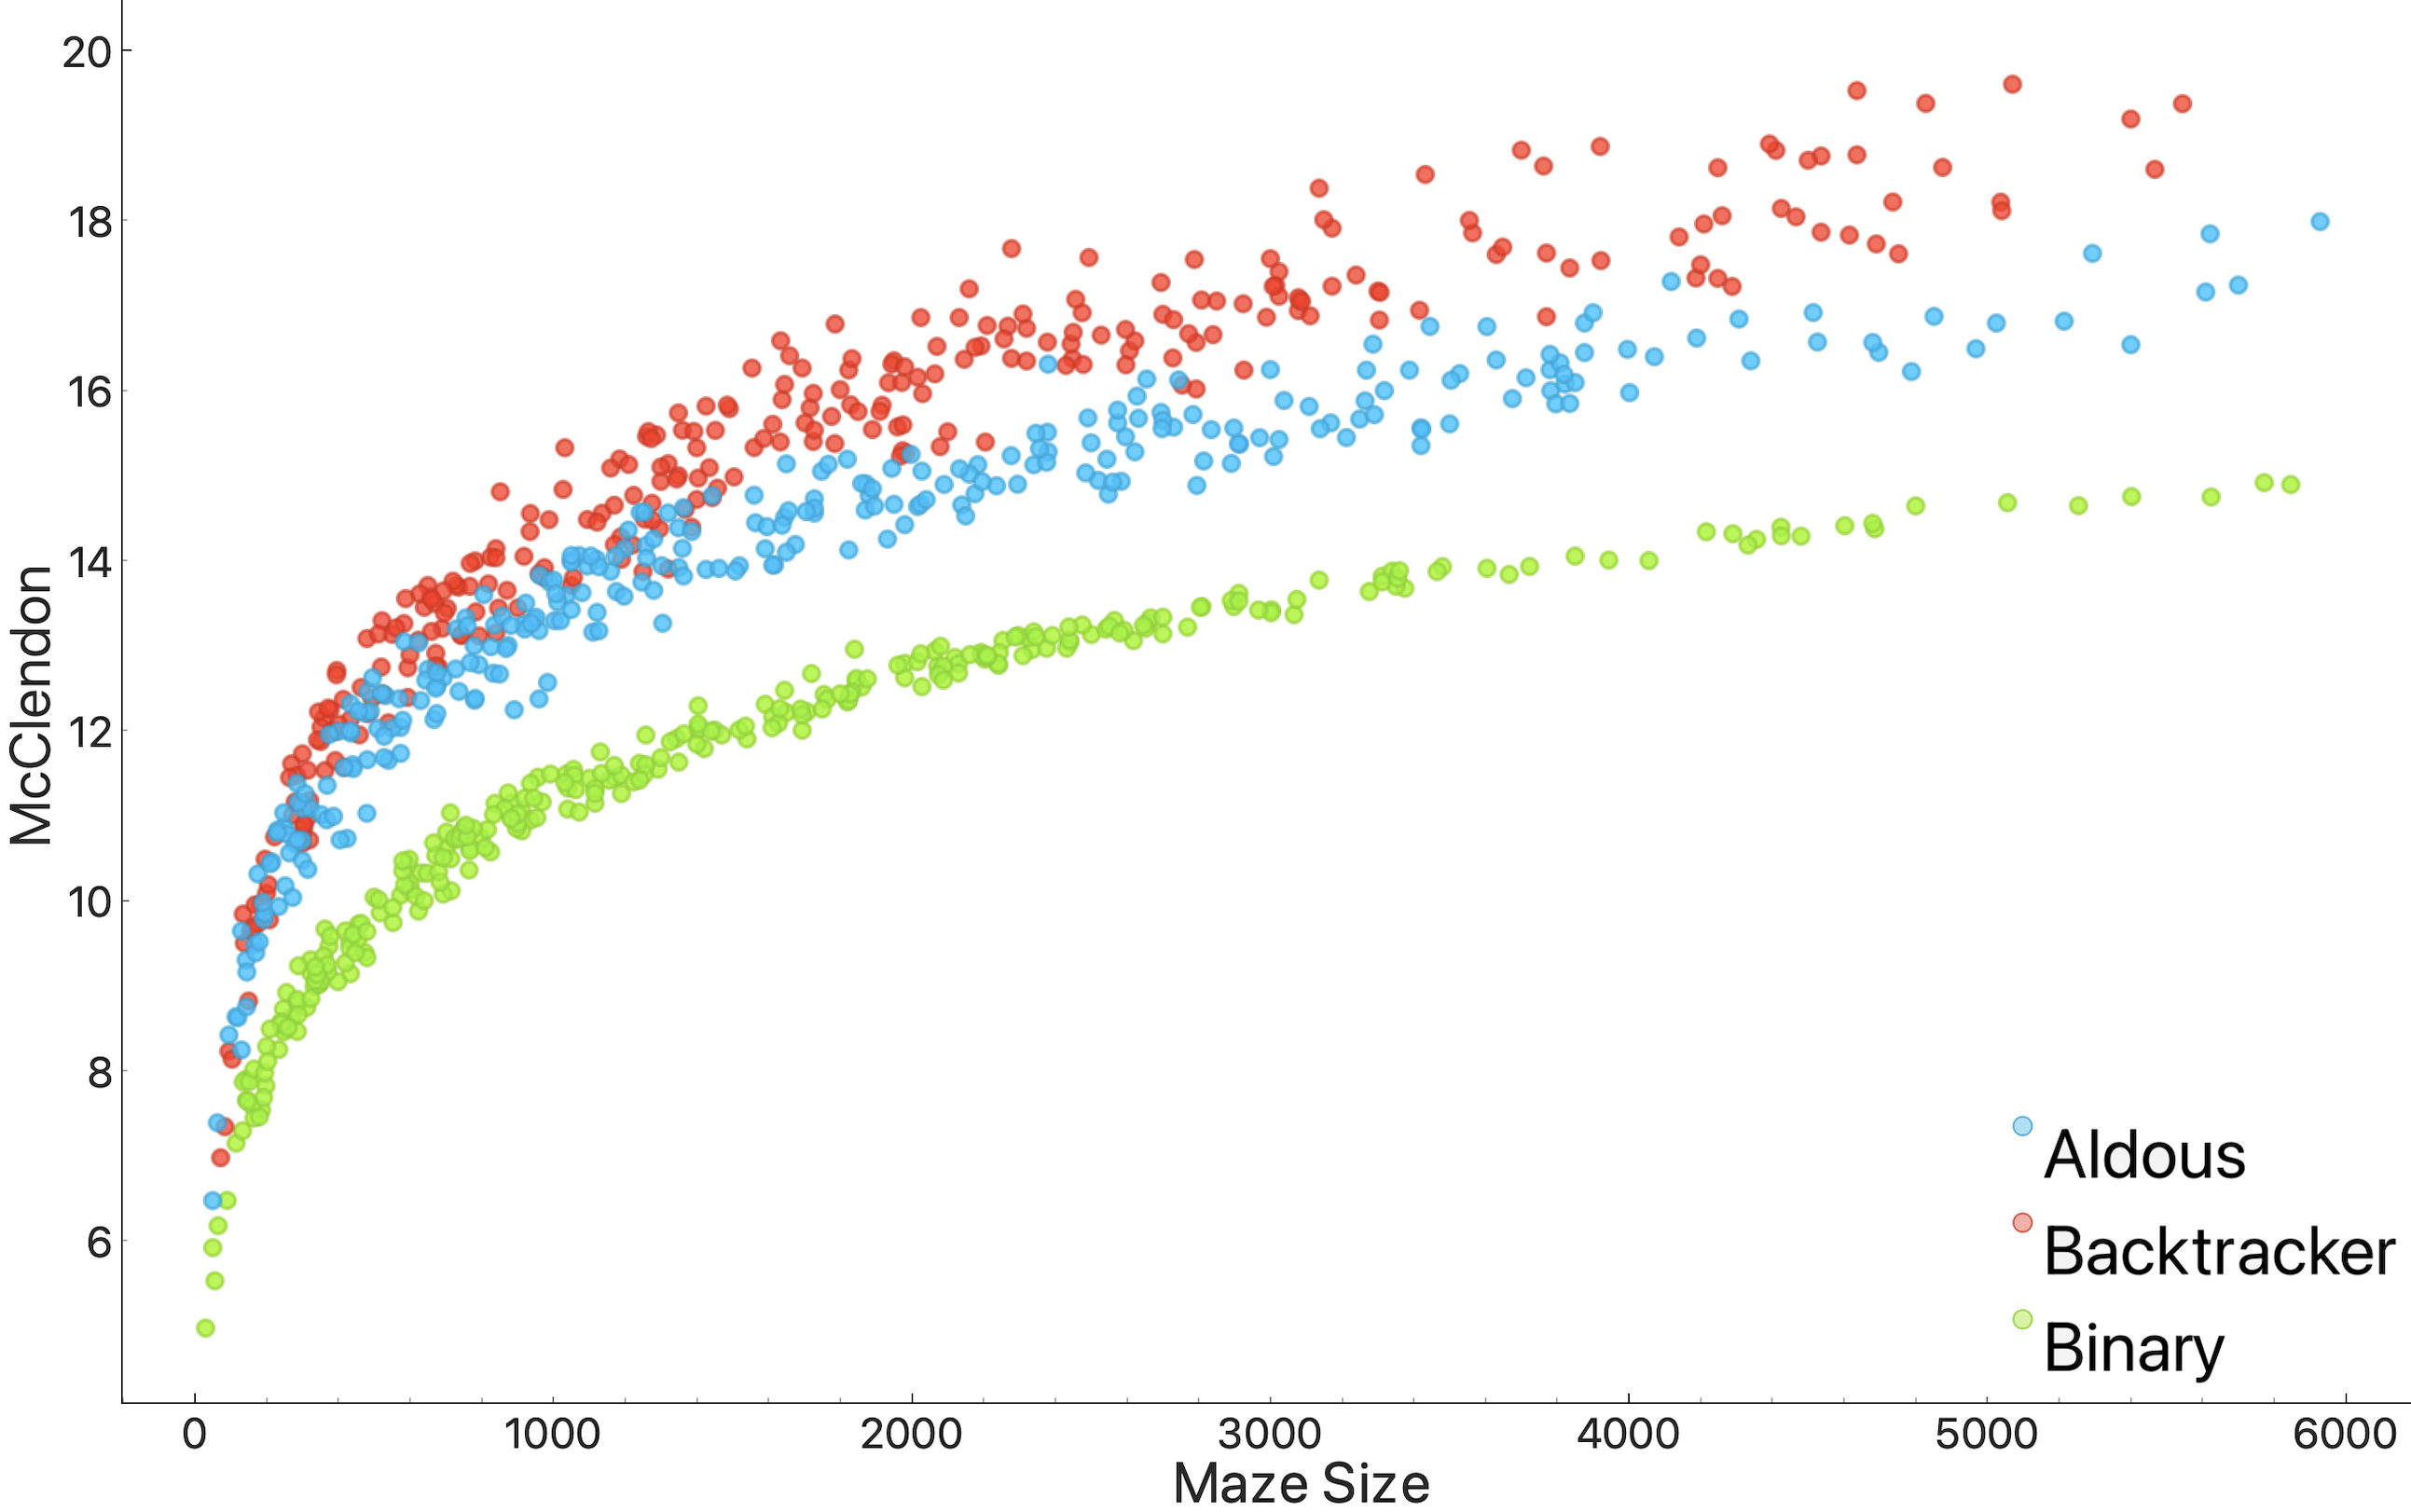
\includegraphics[width=1\linewidth]{MClendon_variant1.png}
               \caption{}
            \end{subfigure}
            \begin{subfigure}[!h]{0.7\textwidth}
               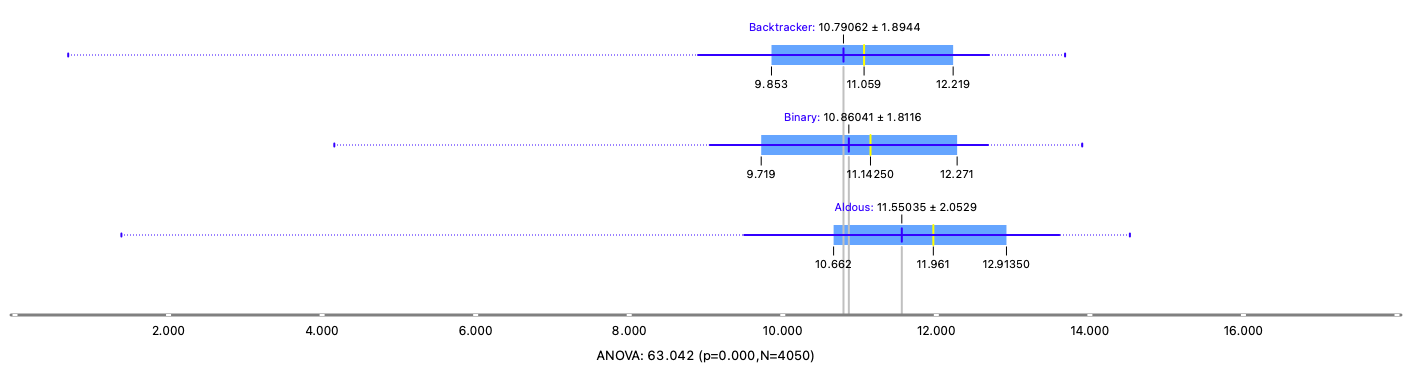
\includegraphics[width=1\linewidth]{McClendon_variant2.png}
               \caption{}
            \end{subfigure}
            \caption{(a) presents Variant 1 and (b) presents Variant 2: a scatter plot of maze size versus McClendon's complexity.}
            \end{figure}%
 %------------------------------------SHANONS ENTROPY---------------------------------------------------------
\subsubsection{Shanonn's Entropy}
Tables 5.8 and 5.9 present the average and median of the complexity measure for different maze generators. Despite the skewness is smaller than 1.5 and stating that the set
distribution is close to the normal distribution, due to huge SD the median may be considered a more reliable measure. In Figures 5.3a and 5.3b, scatter
plots of maze size versus Shannon's entropy are presented.\\

\begin{table}[!ht]
    \centering
    \caption{Variant 1: .} 
    \begin{tabular}{c c c c c c}
    \hline
        Maze Generator & Average & SD & Median & Skewness & W \\ \hline
        Aldous & 1462 & 1125 & 1125 & 0.86 & 0.916  \\ 
        Binary & 1324 & 1074 & 1015 & 1.14 & 0.894  \\ 
        Recursive & 1696 & 1264 & 1369 & 0.809 & 0.920 \\ \hline
    \end{tabular}
\end{table}

\begin{table}[!ht]
    \centering
    \caption{Variant 2: .} 
    \begin{tabular}{cccccc}
    \hline
        Maze Generator & Average & SD & Median & Skewness & W  \\ \hline
        Aldous & 1802 & 1429 & 1466 & 0.926 & 0.909 \\ 
        Binary & 1845 & 1506 & 1468 & 0.931 & 0.901\\ 
        Recursive & 1913 & 1562 & 1512 & 1.061 & 0.897\\ \hline
    \end{tabular}
\end{table}

\begin{figure}[!h]
    \centering
    \begin{subfigure}[!h]{0.7\textwidth}
       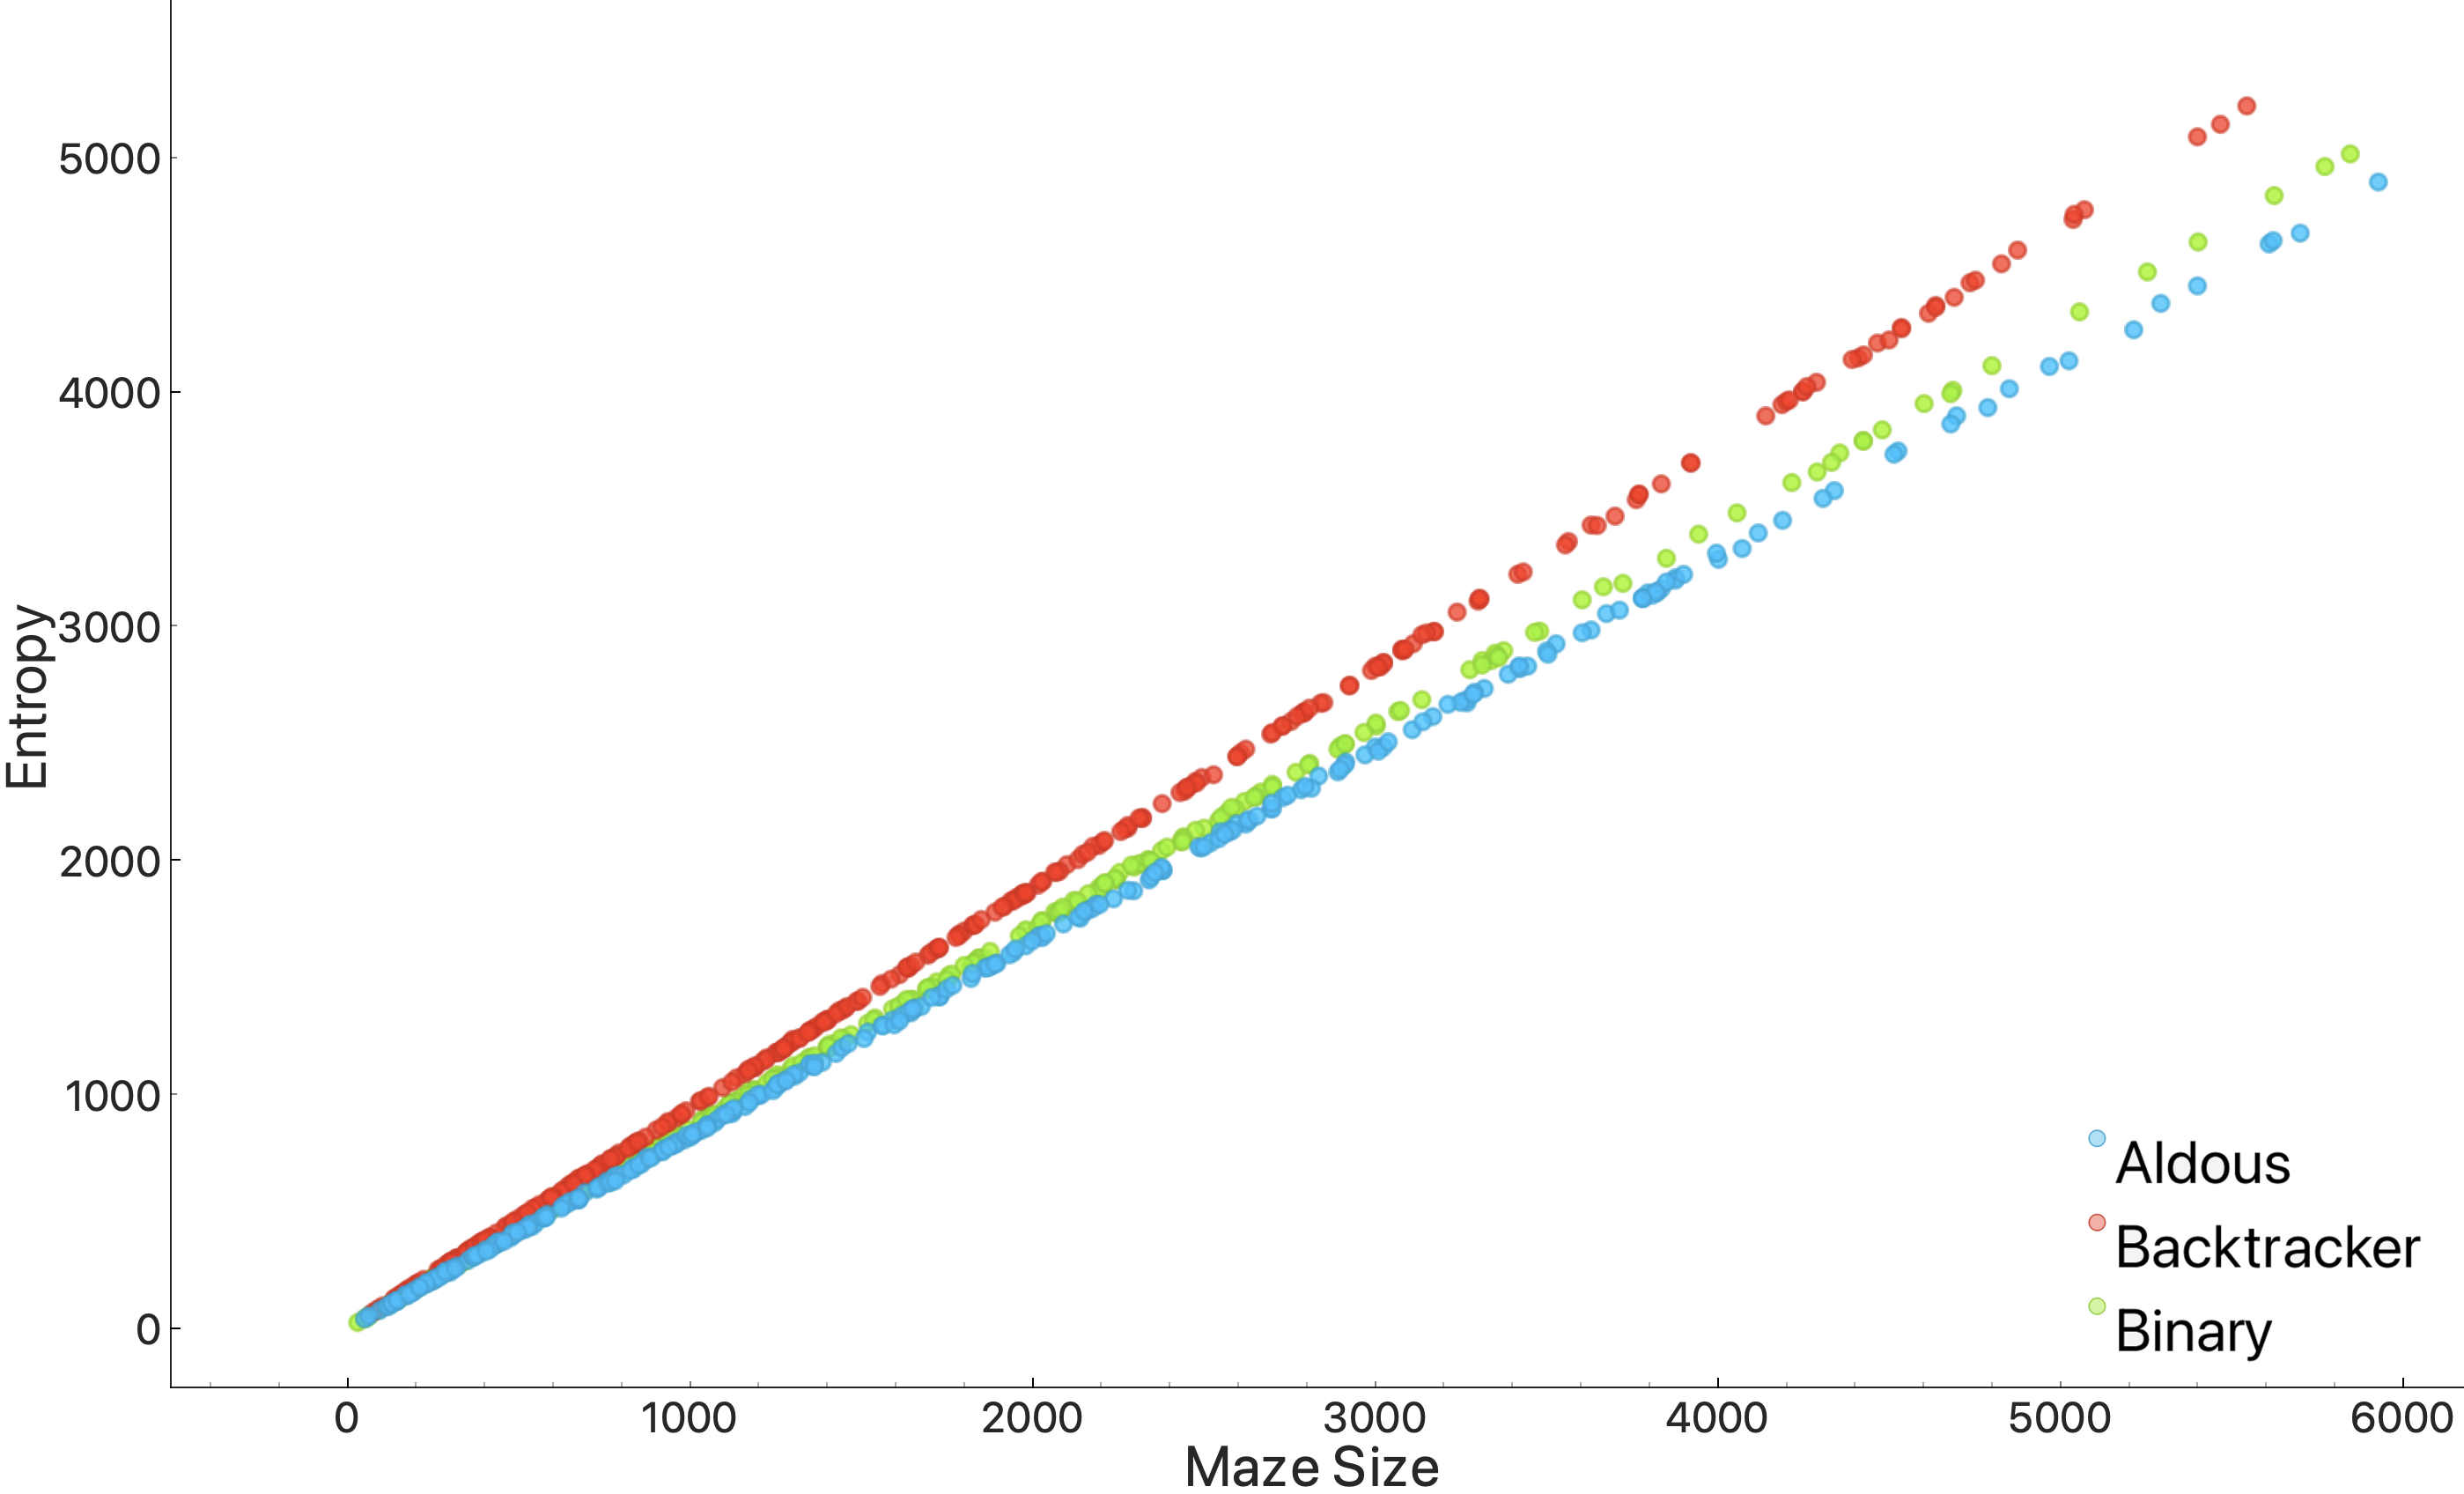
\includegraphics[width=1\linewidth]{entropy_variant1.png}
       \caption{}
    \end{subfigure}
    \begin{subfigure}[!h]{0.7\textwidth}
       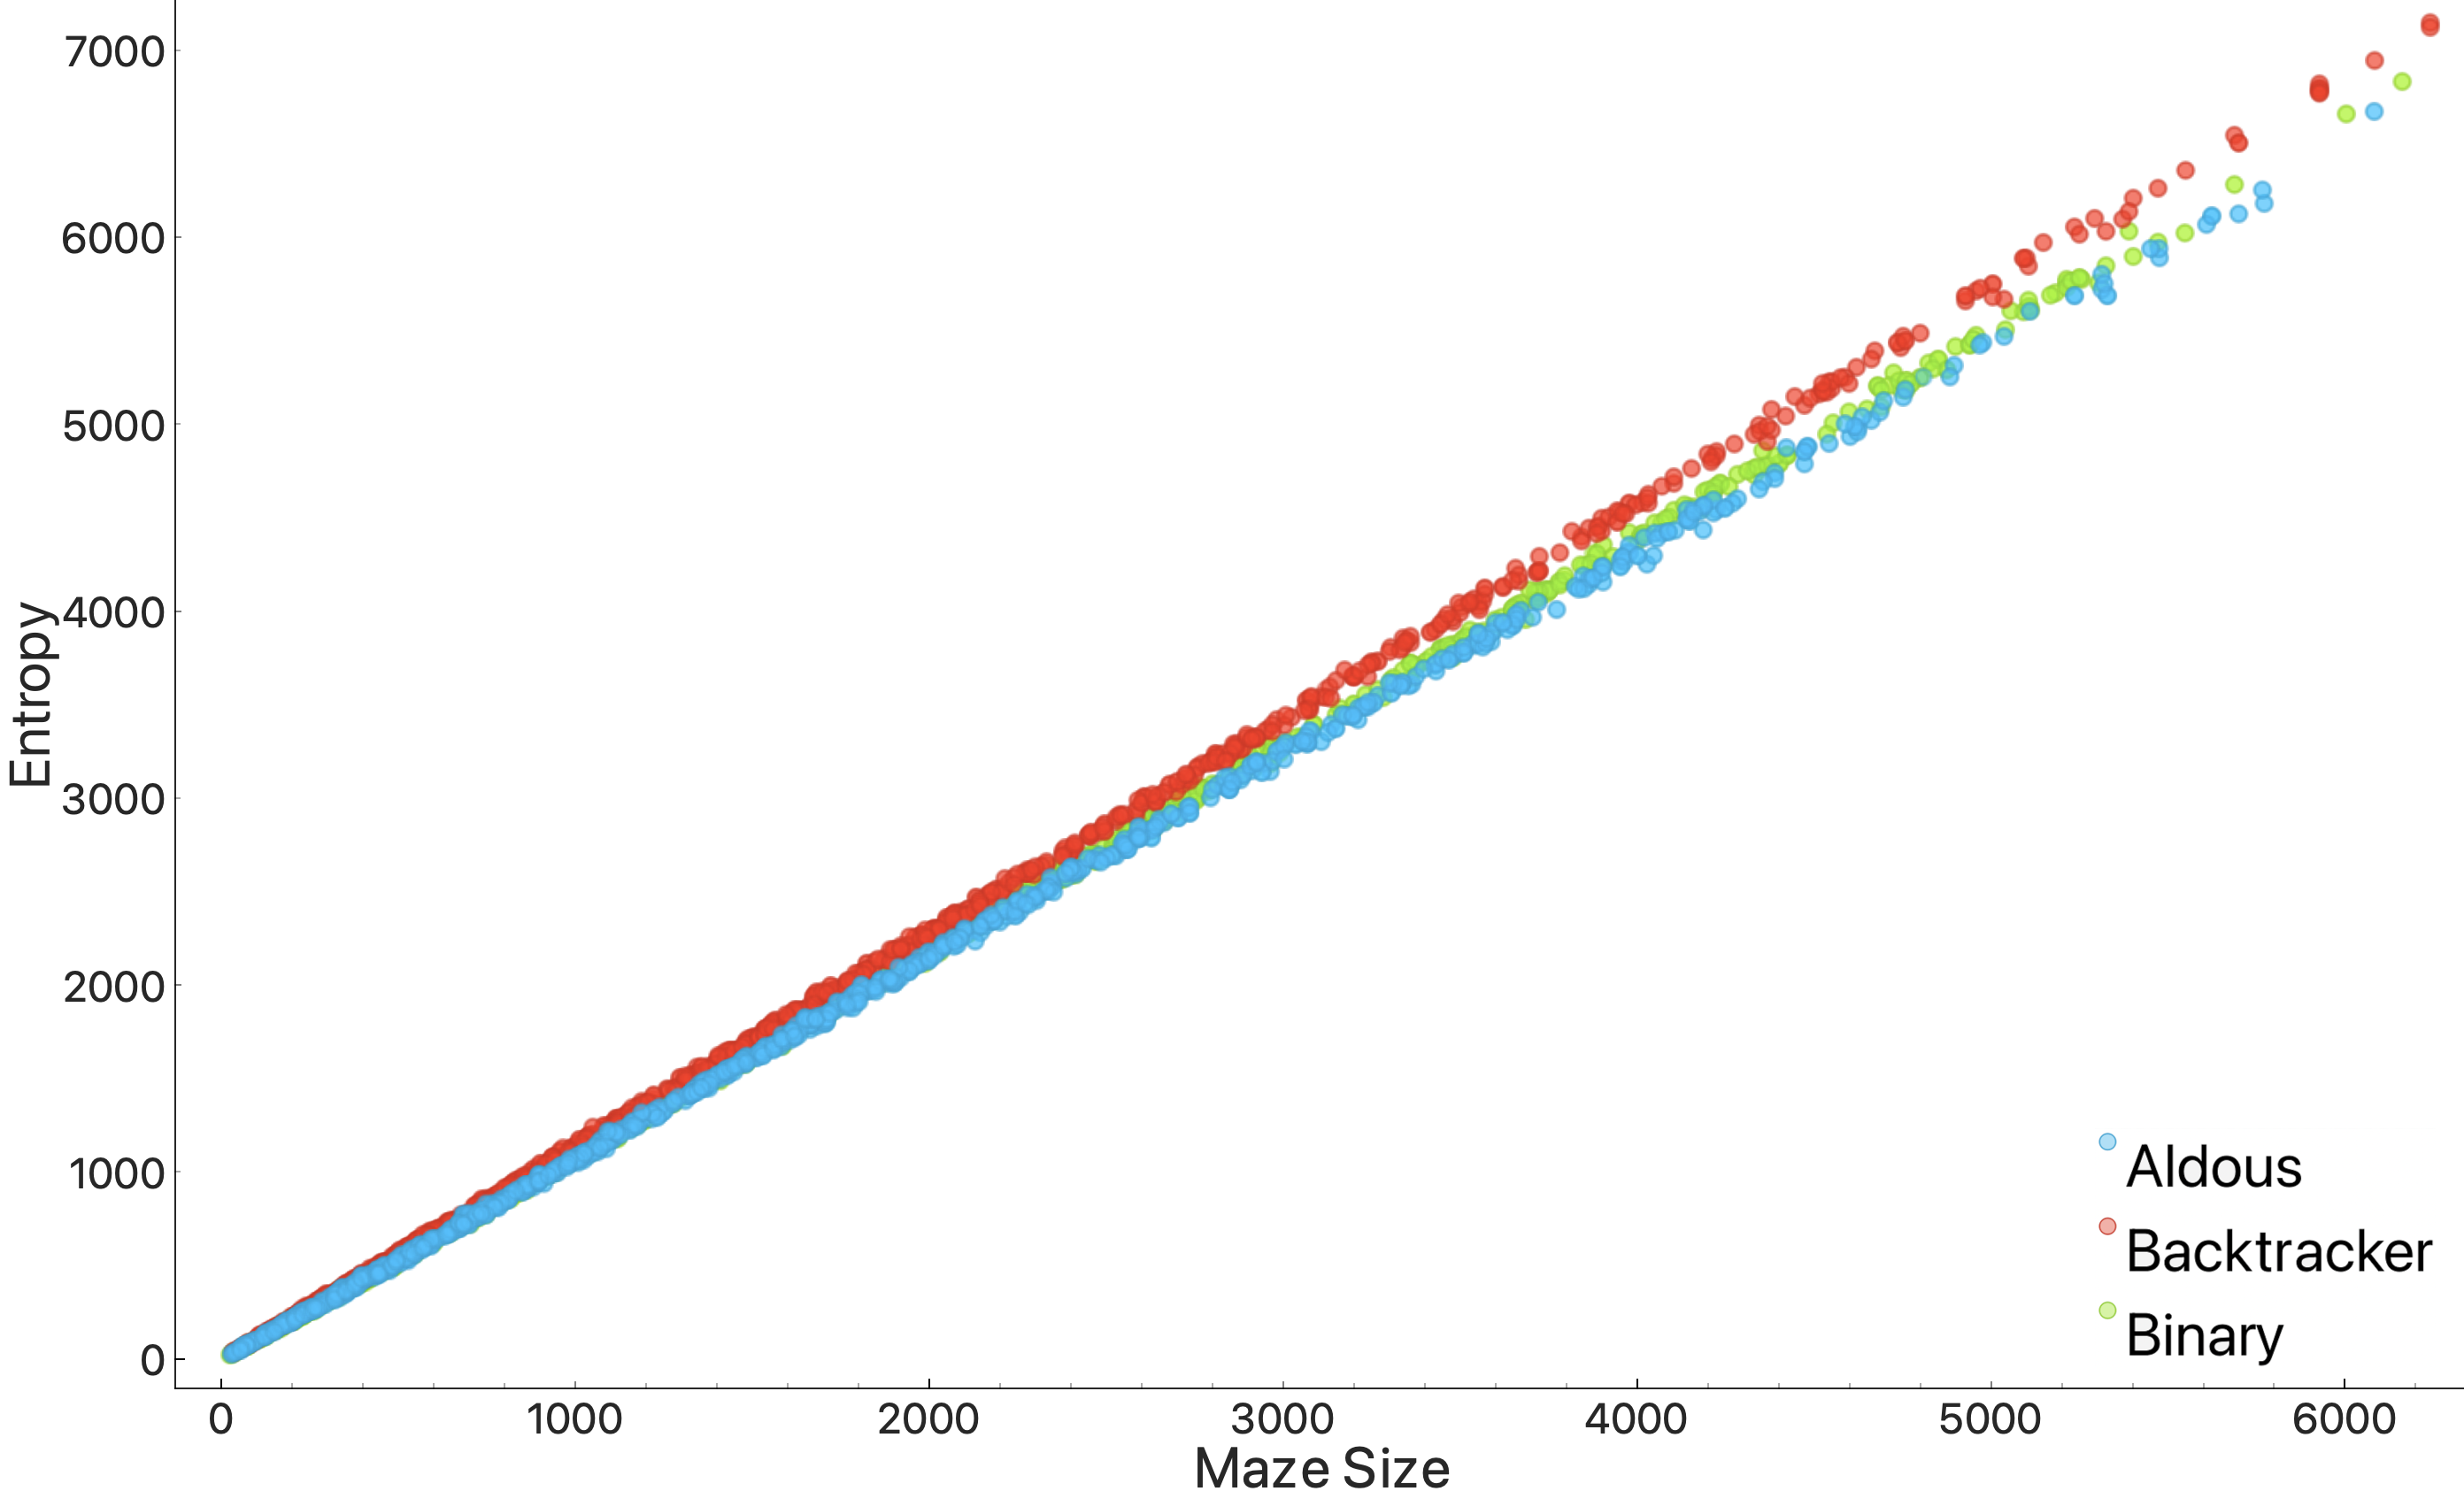
\includegraphics[width=1\linewidth]{entropy_variant2.png}
       \caption{}
    \end{subfigure}
    \caption{(a) presents Variant 1 and (b) presents Variant 2: a scatter plot of maze size versus Shannon's entropy.}
    \end{figure}%
\newpage
%------------------------------------DEGREE DISTRIBUTION--------------------------------------
\subsubsection{Degree Distribution}  
In Tables 5.10 and 5.11 statistical information of degree distribution for different maze generators. Degree distribution for both, variant 1 and variant 2
is defined by the normal distribution so the average and SD may be considered reliable measures.
Figures 5.4a and 5.4b present a scatter plot of a dead-end ratio versus a cross-ratio.

\begin{table}[!h]
    \begin{center} 
        \caption{Variant 1: Degree distribution for different maze generators: Binary Tree, Aldous-Broder and Recursive-Backtracker} 
    \begin{tabular}{ c c c c} 
    \multicolumn{4}{c}{Maze Generator} \\
    \hline
Degree Distribution&Aldous-Broder&Recursive-Backtracker&Binary Tree\\
    \hline
Deadend Ratio&$0.291\pm 0.011$&$0.1021\pm 0.0065$&$0.2512\pm 0.0097$\\    
    \hline
Fork Ratio&$0.455\pm 0.020$&$0.800\pm 0.012$&$0.501\pm 0.019$\\
    \hline
Intersection Ratio&$0.220\pm 0.011$&$0.096\pm 0.011$&$0.248\pm 0.010$\\    
    \hline
Cross Ratio&$0.034\pm 0.006$&$0.001\pm 0.001$&$0.000\pm 0.000$\\    
    \hline   
     \end{tabular} 
    \end{center}
     \end{table}

     \begin{table}[!h]
        \begin{center} 
            \caption{Variant 2: Degree distribution for different maze generators: Binary Tree, Aldous-Broder and Recursive-Backtracker} 
        \begin{tabular}{ c c c c} 
        \multicolumn{4}{c}{Maze Generator} \\
        \hline
    Degree Distribution&Aldous-Broder&Recursive-Backtracker&Binary Tree\\
        \hline
    Deadend Ratio&$0.169\pm 0.025$&$0.067\pm 0.013$&$0.146\pm 0.017$\\    
        \hline
    Fork Ratio&$0.427\pm 0.034$&$0.575\pm 0.026$&$0.436\pm 0.019$\\ 
        \hline
    Intersection Ratio&$0.328\pm 0.025$&$0.325\pm 0.024$&$0.361\pm 0.021$\\   
        \hline
    Cross Ratio&$0.077\pm 0.021$&$0.034\pm 0.010$&$0.057\pm 0.010$\\   
        \hline   
         \end{tabular} 
        \end{center}
         \end{table}
         \begin{figure}[!h]
            \centering
            \begin{subfigure}[!h]{0.7\textwidth}
                \includegraphics[width=1\linewidth]{crossvSDeas_variant1.png}
               \caption{}
            \end{subfigure}
            \begin{subfigure}[!h]{0.7\textwidth}
                \includegraphics[width=1\linewidth]{crossvSDead_variant2.png}
               \caption{}
            \end{subfigure}
            \caption{(a) presents Variant 1 and (b) presents Variant 2: A scatter plot of dead-end ratio versus cross-ratio.}
            \end{figure}

\section{Practical analysis of maze generators and maze solvers}
In this section, all algorithms described in Chapter 4 are assessed in terms of their runtime and parameters of generated solutions. Three algorithms described
in Chapter 4 were evaluated: Dijkstra, $A^*$ and BFS, each algorithm was tested in the same way. The runtime measurement program worked as follows,
the program generated a random-sized maze using one of the three algorithms: Binary Tree, Recursive Backtracker and Aldous-Broder. Then each solving
algorithm one by one was applied to solve the same problem. Mazes were generated with randomly assigned sizes ranging from $5 \times 5$ to $80 \times 80$.
The main assumption was to create a rectangular maze with the source cell $p$ at the left top corner, and the goal cell $q$ at the right bottom corner of the maze grid. 
All solvers could only use the NSWE moves described in Chapter 4. Maze problems usually have quick access to basic heuristic functions because of
a graph implemented as a grid. Because of the assumption that only the NSWE moves are allowed the heuristic method $h(v)$ applied in algorithm $A^*$ was the
Manhattan Distance.
The purpose is to compare both the maze generators and the solvers and build a framework which could classify which algorithms comply best with each other.
Although the runtime of both, the generating and solving algorithms were measured, it was not the purpose of this work to minimize it. Therefore, the algorithms
were implemented in JavaScript. It is beyond discussion that the implementation in a more low-level language would be more efficient, and could lead to building
and solving bigger mazes. However, the choice of using Java Script for algorithm implementation was dictated by the eagerness of building a web application
depending on and harnessing the results of this work. 
The reprezentative set of solved mazes is presented in Figure 5.5.%tutaj dołozyć inne rodzaje mazów
\begin{figure}[!h]
	\centering
	\begin{subfigure}{.30\textwidth}
	  \centering
	  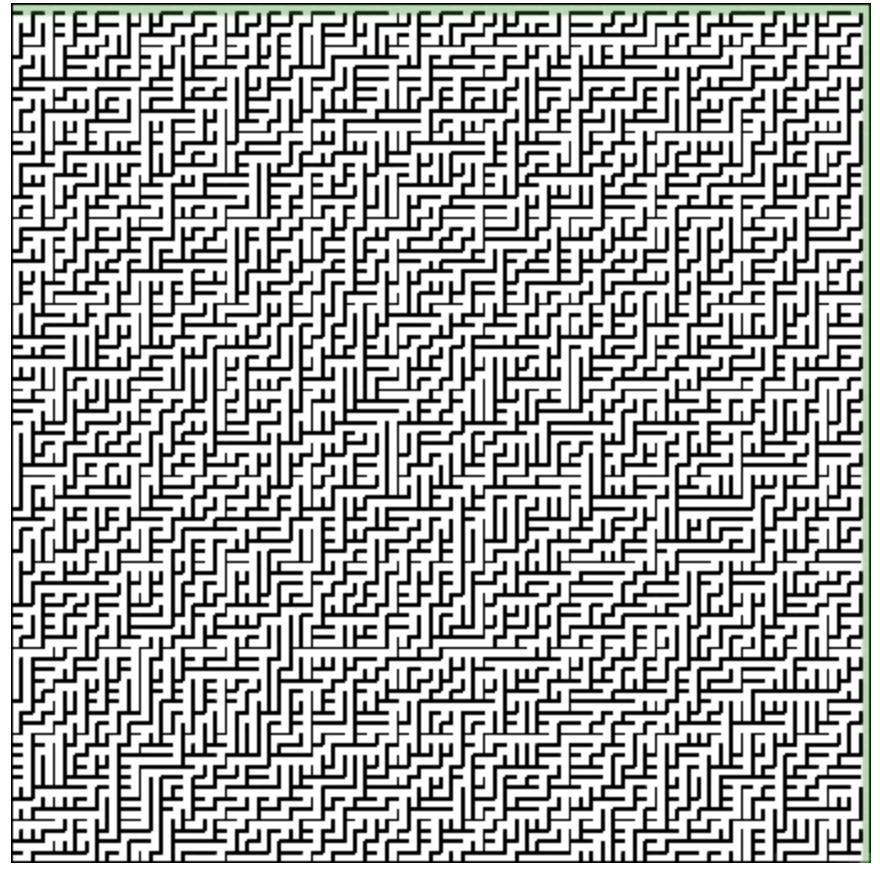
\includegraphics[width=1\linewidth]{perfectBinary.png}
	  \caption{}
	  \label{fig:sub1}
	\end{subfigure}
	\begin{subfigure}{.30\textwidth}
	  \centering
	  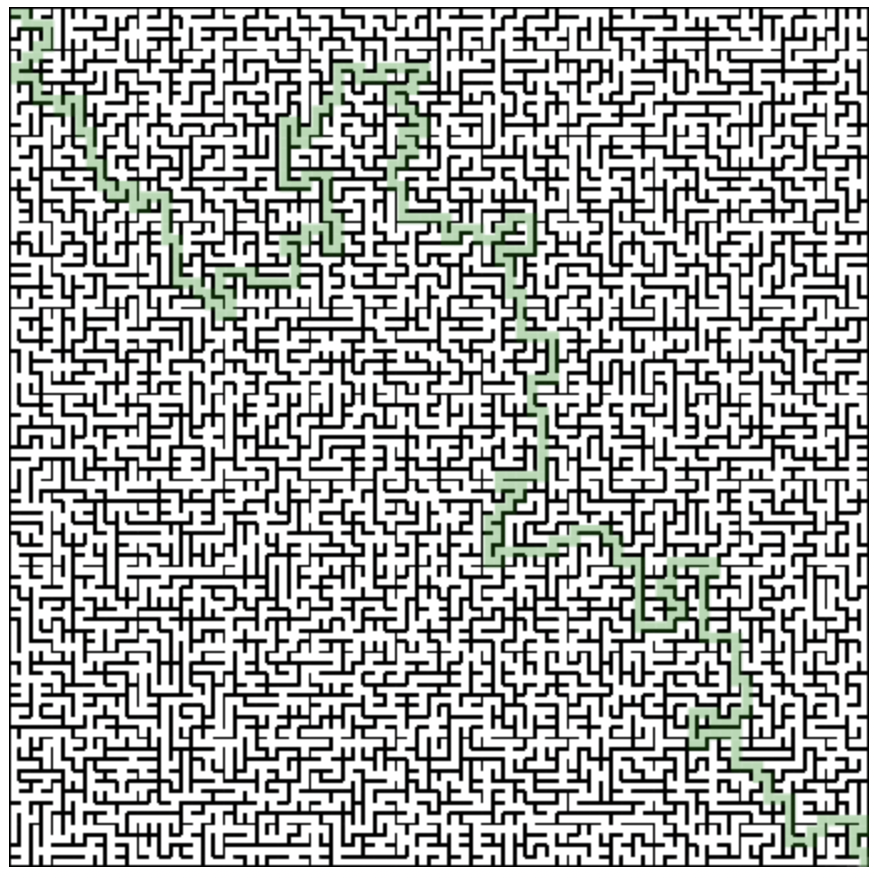
\includegraphics[width=1\linewidth]{perfectAldous.png}
	  \caption{}
	  \label{fig:sub2}
	\end{subfigure}
    \begin{subfigure}{.30\textwidth}
        \centering
        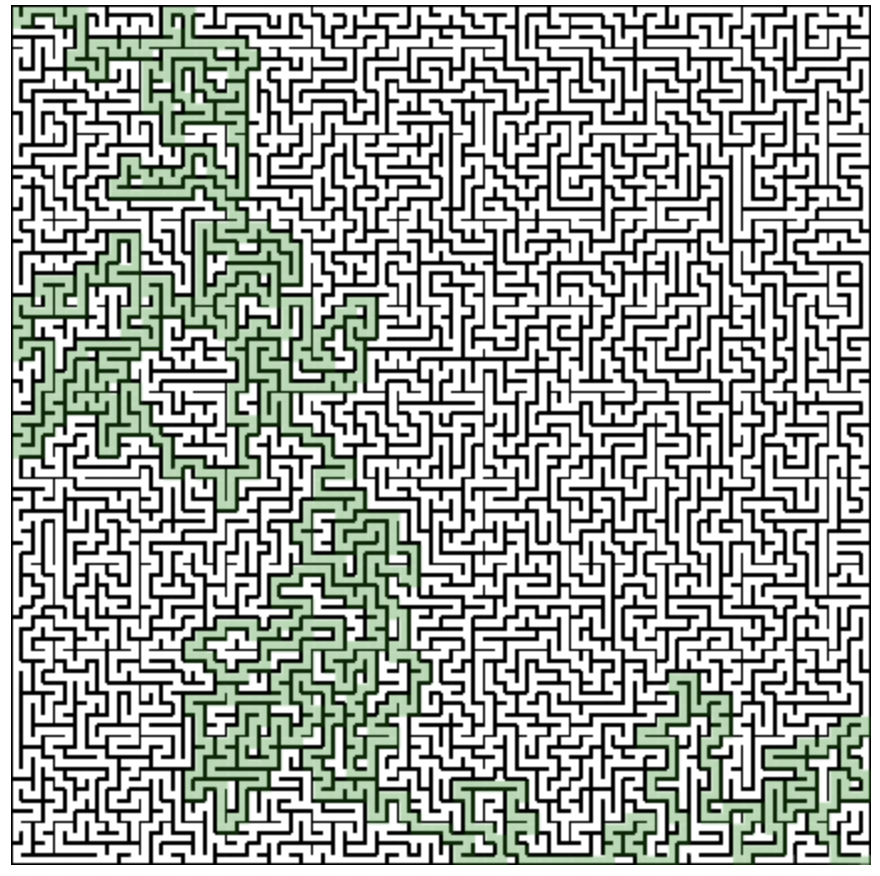
\includegraphics[width=1\linewidth]{perfectRecursive.png}
        \caption{}
        \label{fig:sub2}
      \end{subfigure}
	\caption{Examples of different, perfect,  80 $\times$ 80 mazes with applied Dijkstra solution. In subfigure (a) there is a Binary Tree maze, in (b) an Aldous-Broder maze, and in (c) Recursive-Backtracker
    \\Source: developed by the author}
	\label{fig:test}
	\end{figure}
\subsection{Path and time comparison for different maze solvers - Q1 acknowledgement}
\textbf{Variant 1}\\
\indent The algorithm which generates mazes with the longest path median is Recursive-Backtracker, which is $227$. The shortest average path is generated by
Binary Tree algorithm, which is $59\pm 25$. A significant value of the average path length might indicate a higher number of longer paths in the maze. That 
may results in a longer solution time due to the greater number of long side paths, i.e. paths that are not a solution. This is also confirmed by the results of
the measured number of steps and time, which are also the biggest for Recursive-Backtracker, and the smallest for Binary Tree for every solver as shown in
Tables 5.2, 5.3, 5.4 and 5.5. What is noticeable for this data set is a very big standard deviation, which might be caused by a big maze size range.
The results for Aldous-Broder mazes fall between Recursive-Backtracker and Binary, as well as for solution time, path length and steps needed to solve.\\
\indent Solution time for the Dijkstra solver is the shortest regardless of the size and maze type. Dijkstra's median of solution time does not exceed 0.2 ms for each type of maze.
The longest solution time was measured for Astar solver for which the worst-case is 14.46 ms for solving a Recursive-Backtracker maze.
However, the Astar solution time varies the most depending on the maze generator which is visible in Figure 5.1a and Table 5.4\\
\textbf{Variant 2}\\ 
\indent There is an observable drop in the median of the number of steps and solution time for Astar and BFS solvers in mazes with cycles. Astar, worst-case solution time, 
for a Recursive-Backtracker maze, is only 1.84 ms in comparison to 14.46 ms for a perfect maze. The BFS solution time is also lower than for the perfect mazes, but not
that significant. BFS worst-case solution time for a Recursive-Backtracker maze is 0.89 ms in comparison to 1.14 ms for a perfect maze. 
The Dijkstra algorithm was the fastest solver for all maze generators.\\
\indent The presented results in some way contradict the conclusions contained in the paper \cite{31}, where the authors examined the same solvers but 
only small and medium-sized grids, with a maximum size of 32x32 and only square ones. The popular opinion \cite{32} that the $A^*$ algorithm must always be the fastest solver wasn't
confirmed in this work. The additional calculations which Astar is performing while searching the solutions in the case of this work, significantly increased
the solution time. It is true that the number of steps performed is lower compared to other solvers in the case of mazes with cycles and directed,
but this does not affect the time of the solution.\\
\subsection{Analysis of parameters affecting maze complexity - Q2 acknowledgement}
\textbf{Variant 1}\\
\indent The evaluation of McClendon's complexity shows that the three types of maze generators can be characterized by this measure. The results confirm the conclusions
of path and solution time evaluation. The most complex maze type is a Recursive-Backtracker with average complexity equal to $14.94 \pm 2.48$, the easiest type is 
Binary-Tree with average complexity equals $11.36 \pm 1.98$. The McClendon's complexity is based on hallway length so the results are consistent with what was said earlier about
Recursive-Backtracker mazes.\\
Another complexity measure which has the potential to assess maze complexity is Shannon's entropy. There are few sources applying entropy to the mazes problems,
as entropy is rather considered for bigger networks. However, besides the big standard deviation, Shannon's entropy seems to correctly evaluate maze complexity
in terms of its solution time. Figure 5.3a presents the data for maze entropy versus maze size. The relation is linear, however, each maze type can be easily distinguished.
Moreover, the hierarchy of entropy corresponds to solution time. The bigger the entropy the longer the solution time. The most difficult mazes are Recursive-Backtracker and 
the easiest are Binary Trees. The implemented entropy is based not on the length path but rather a degree distribution, which allows concluding that it is the most reliable 
maze complexity measure that McClendon's.\\
\textbf{Variant 2}\\
On the other hand, McClendon's complexity measure does not occur accurately for mazes with cycles. Figure 5.2b and Table 5.7 state that the most
complicated mazes are Aldous-Broder, Binary Tree and the easiest Recursive-Backtracker. But the solution times for each solver are the lowest, particularly for 
Aldous-Broder mazes. It seems that the McClendon complexity measure does not reflect the actual complexity but rather the hallway lengths and their twistiness. So it
is tightly connected only to maze size, without taking into consideration the complexity itself.
Which was also proven in \cite{4}, and confirmed by this work for a cyclic mazes.\\
Shannon's entropy was also measured for cycled and directed mazes, and the results are also very satisfying. The entropy level corresponds firmly with a solution time.
The results are even better than for the perfect mazes. Different types of mazes can be even better predicted by this entropy measure.
Furthermore, this is the only measure which manifests higher complexity to mazes with added cycles and direction. It s meaningful because it represents, the 
more complex state of the maze both statistically but also algorithmically.
\subsection{Parametrizing the maze problem for choosing the best solver - Q3 acknowledgement}
The parameters described so far did not allow for a clear distinction between different types of mazes. Taking into account the data collected in Tables 5.10, 5.11 and Figures 5.4a and 5.4b,
we can conclude that the most accurate measure of distinguishing between mazes is the cross number to a dead-end number ratio.
Figure 5.4a shows how well different types of mazes can be distinguished on this basis. Despite, that the split between Aldous-Broder and Binary Tree
mazes with cycles presented in Figure 5.4b is not that well separated, the mazes can still be distinguished. 
The separation classes could be defined by functions as follows: for variant 1 cross ratio $< 0.01$ and dead-end ratio $< 0.14$ denotes BackTracker maze,
cross ratio $= 0$ denotes Binary tree maze in this configuration, dead-end ratio $> 0.25$ and cross ratio $> 0$ denotes Aldous-Broder maze.
For variant 2 cross ratio$ < -6.67\cdot$dead-end ratio $+ 0.8$ denotes Backtracker maze, cross-ratio $< -0.48\cdot$dead-end ratio $+0.14$ denotes Binary Tree maze, 
and cross ratio$ > -0.4\cdot$dead-end ratio +0.14 indicates the Aldous-Broder maze.
Despite a lot of work dedicated to studying the degree distribution, non of them tries to apply such measures to introduce a framework to distinguish mazes by it.
As was already proven the best maze solver for the perfect mazes generated by Binary Tree, Aldous-Broder and Recursive-Backtracker is the Dijkstra algorithm.
The best solver for studied mazes with cycles and directed edges was Dijkstra for all maze generators.
\section{Conclusions}
This section presents the conclusions of the presented results and analysis. This thesis was an attempt to create a basic framework which could be helpful
for researchers, engineers and developers to have a better understanding of maze problems. Three generating and solving algorithms were tested. Seven 
maze parameters were evaluated along with two different complexity measures. It was possible to compare obtained data with other works. After the results of analysis and 
discussion the answers to the research question are submitted:
\begin{enumerate}
    \item [Q1.] What is the relation between the maze features, generated by Binary Tree, Aldous-Broder and Recursive-Backtracker algorithms,
     and their completion time obtained, when solved using a BFS, Dijkstra and $A^*$ algorithms?\\
     Solution time for perfect mazes with longer subsidiary paths, and cycled-directed mazes with higher fork and intersection ratios, such as Binary Tree,
     identify to have longer solution time.
    \item [Q2.] Which maze parameters best describe the complexity of a problem in terms of time completion?\\
    Shanon's Entropy seems to be the most accurate predicate of maze complexity, independent of maze size. 
    \item [Q3.] Which maze features are the best to distinguish different types of mazes?\\
    The best maze feature to distinguish Binary Tree, Aldous-Broder and Recursive-Backtracker is cross number to dead-end number, both 
    for perfect mazes and mazes with added cycles and directions.
\end{enumerate} 

